\chapter{Avaliação no conjunto de teste e custo versus efetividade}
\label{cap:teste}

\section{Desempenho e custo dos modelos finais}
\label{sec:finais}

Treinados com toda a base de treino e avaliados no teste, M1 e M2 empatam em Macro F1 (0,6065) e M3 fica 0,002 abaixo (Tabela~\ref{tab:finais} e Figura~\ref{fig:custo}). M1 também teve o melhor Macro F1 de validação (0,6046); com uma única semente por modelo, diferenças dessa ordem não são significativas, e o fator decisivo é o custo: M1 foi escolhido por ter o mesmo desempenho com a menor rede (28\% menos parâmetros que M2, uma única camada oculta) e um quinto do tempo de treino de M2. A inferência é desprezível nos três: cerca de 0,1 s para 334 mil acidentes em CPU.

\begin{table}[!htbp]
\caption{Desempenho e custo dos modelos finais no teste}
\label{tab:finais}
\begin{center}
\scriptsize
\setlength{\tabcolsep}{4pt}
\begin{tabular}{cccccccccc}
\hline
\textbf{Modelo} & \textbf{Parâmetros} & \makecell{\textbf{Épocas}\\\textbf{(melhor)}} & \makecell{\textbf{Treino}\\\textbf{(s)}} & \makecell{\textbf{Inferência}\\\textbf{(ms)}} & \textbf{Acurácia} & \makecell{\textbf{Precisão}\\\textbf{macro}} & \makecell{\textbf{\textit{Recall}}\\\textbf{macro}} & \textbf{Macro F1} & \makecell{\textbf{Macro F1}\\\textbf{val}} \\ \hline
\textbf{M1} & 34.059 & 22 (17) & 119 & 126 & \textbf{0,7029} & 0,6020 & 0,6140 & \textbf{0,6065} & 0,6046 \\
M2 & 47.403 & 13 (8) & 580 & 98 & \textbf{0,7029} & 0,6034 & 0,6142 & \textbf{0,6065} & 0,6041 \\
M3 & 46.499 & 8 (3) & 261 & 98 & 0,7023 & 0,6051 & 0,6077 & 0,6041 & 0,6017 \\ \hline
\end{tabular}
\end{center}
\fontetab{Elaborado pelo autor. Inferência sobre os 333.798 exemplos do teste, em CPU}
\end{table}

\begin{figure}[!htbp]
  \centering
  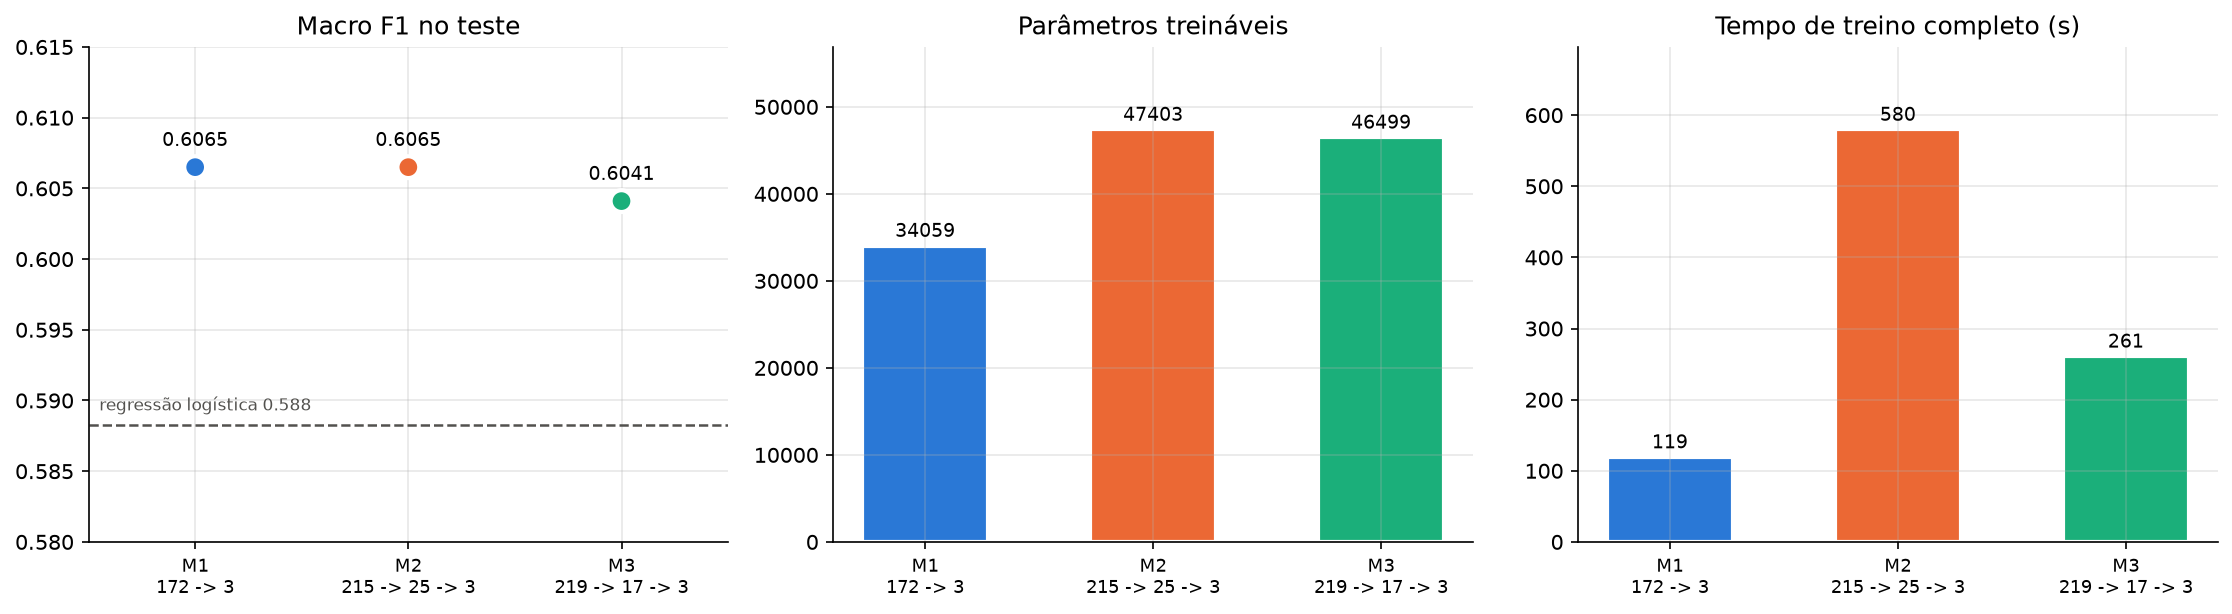
\includegraphics[width=0.65\textwidth]{figuras/18_custo_efetividade}
  \caption{Macro F1 no teste, parâmetros e tempo de treino dos modelos finais}
  \label{fig:custo}
  \fontefig{Elaborado pelo autor}
\end{figure}

A Figura~\ref{fig:confusao} mostra as matrizes de confusão do M1. \texttt{Sem Vítimas} é a classe mais fácil (\textit{recall} de 78\%); o erro mais comum é entre \texttt{Sem Vítimas} e \texttt{Com Vítimas Feridas}, que têm relatos parecidos. Dos acidentes fatais, 40\% são reconhecidos (precisão 0,36, F1 0,38), 46\% vão para \texttt{Com Vítimas Feridas} e 14\% para \texttt{Sem Vítimas}: 86\% dos fatais são sinalizados como \aspas{com vítima}, o que já aciona o socorro, e os 14\% restantes são o erro mais grave do modelo.

\begin{figure}[!htbp]
  \centering
  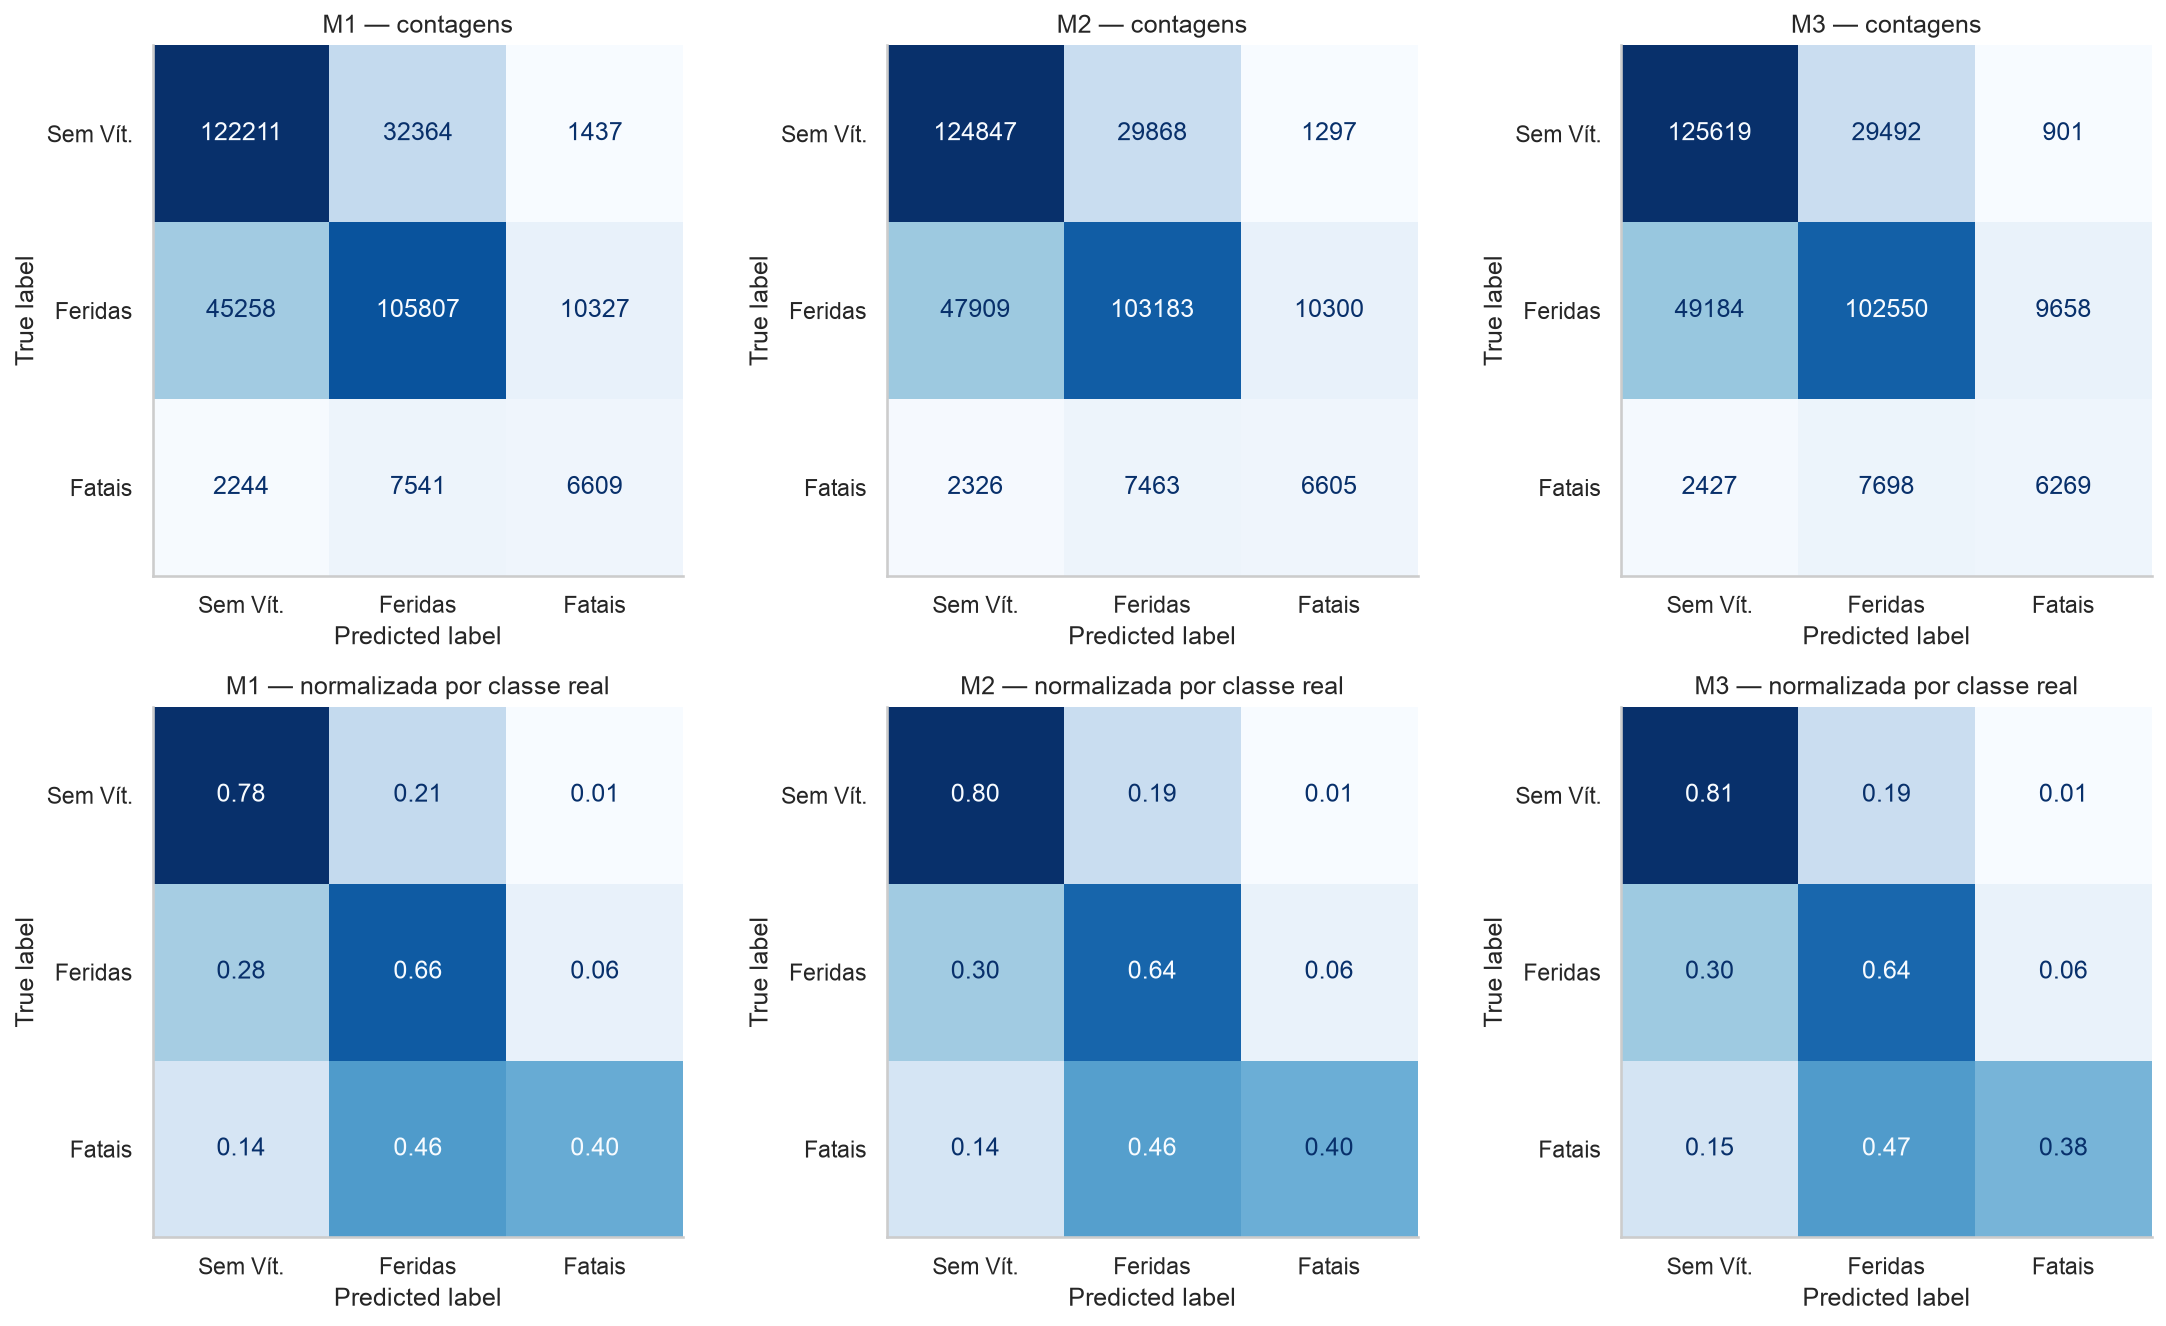
\includegraphics[width=0.5\textwidth]{figuras/11_matrizes_confusao}\hfill
  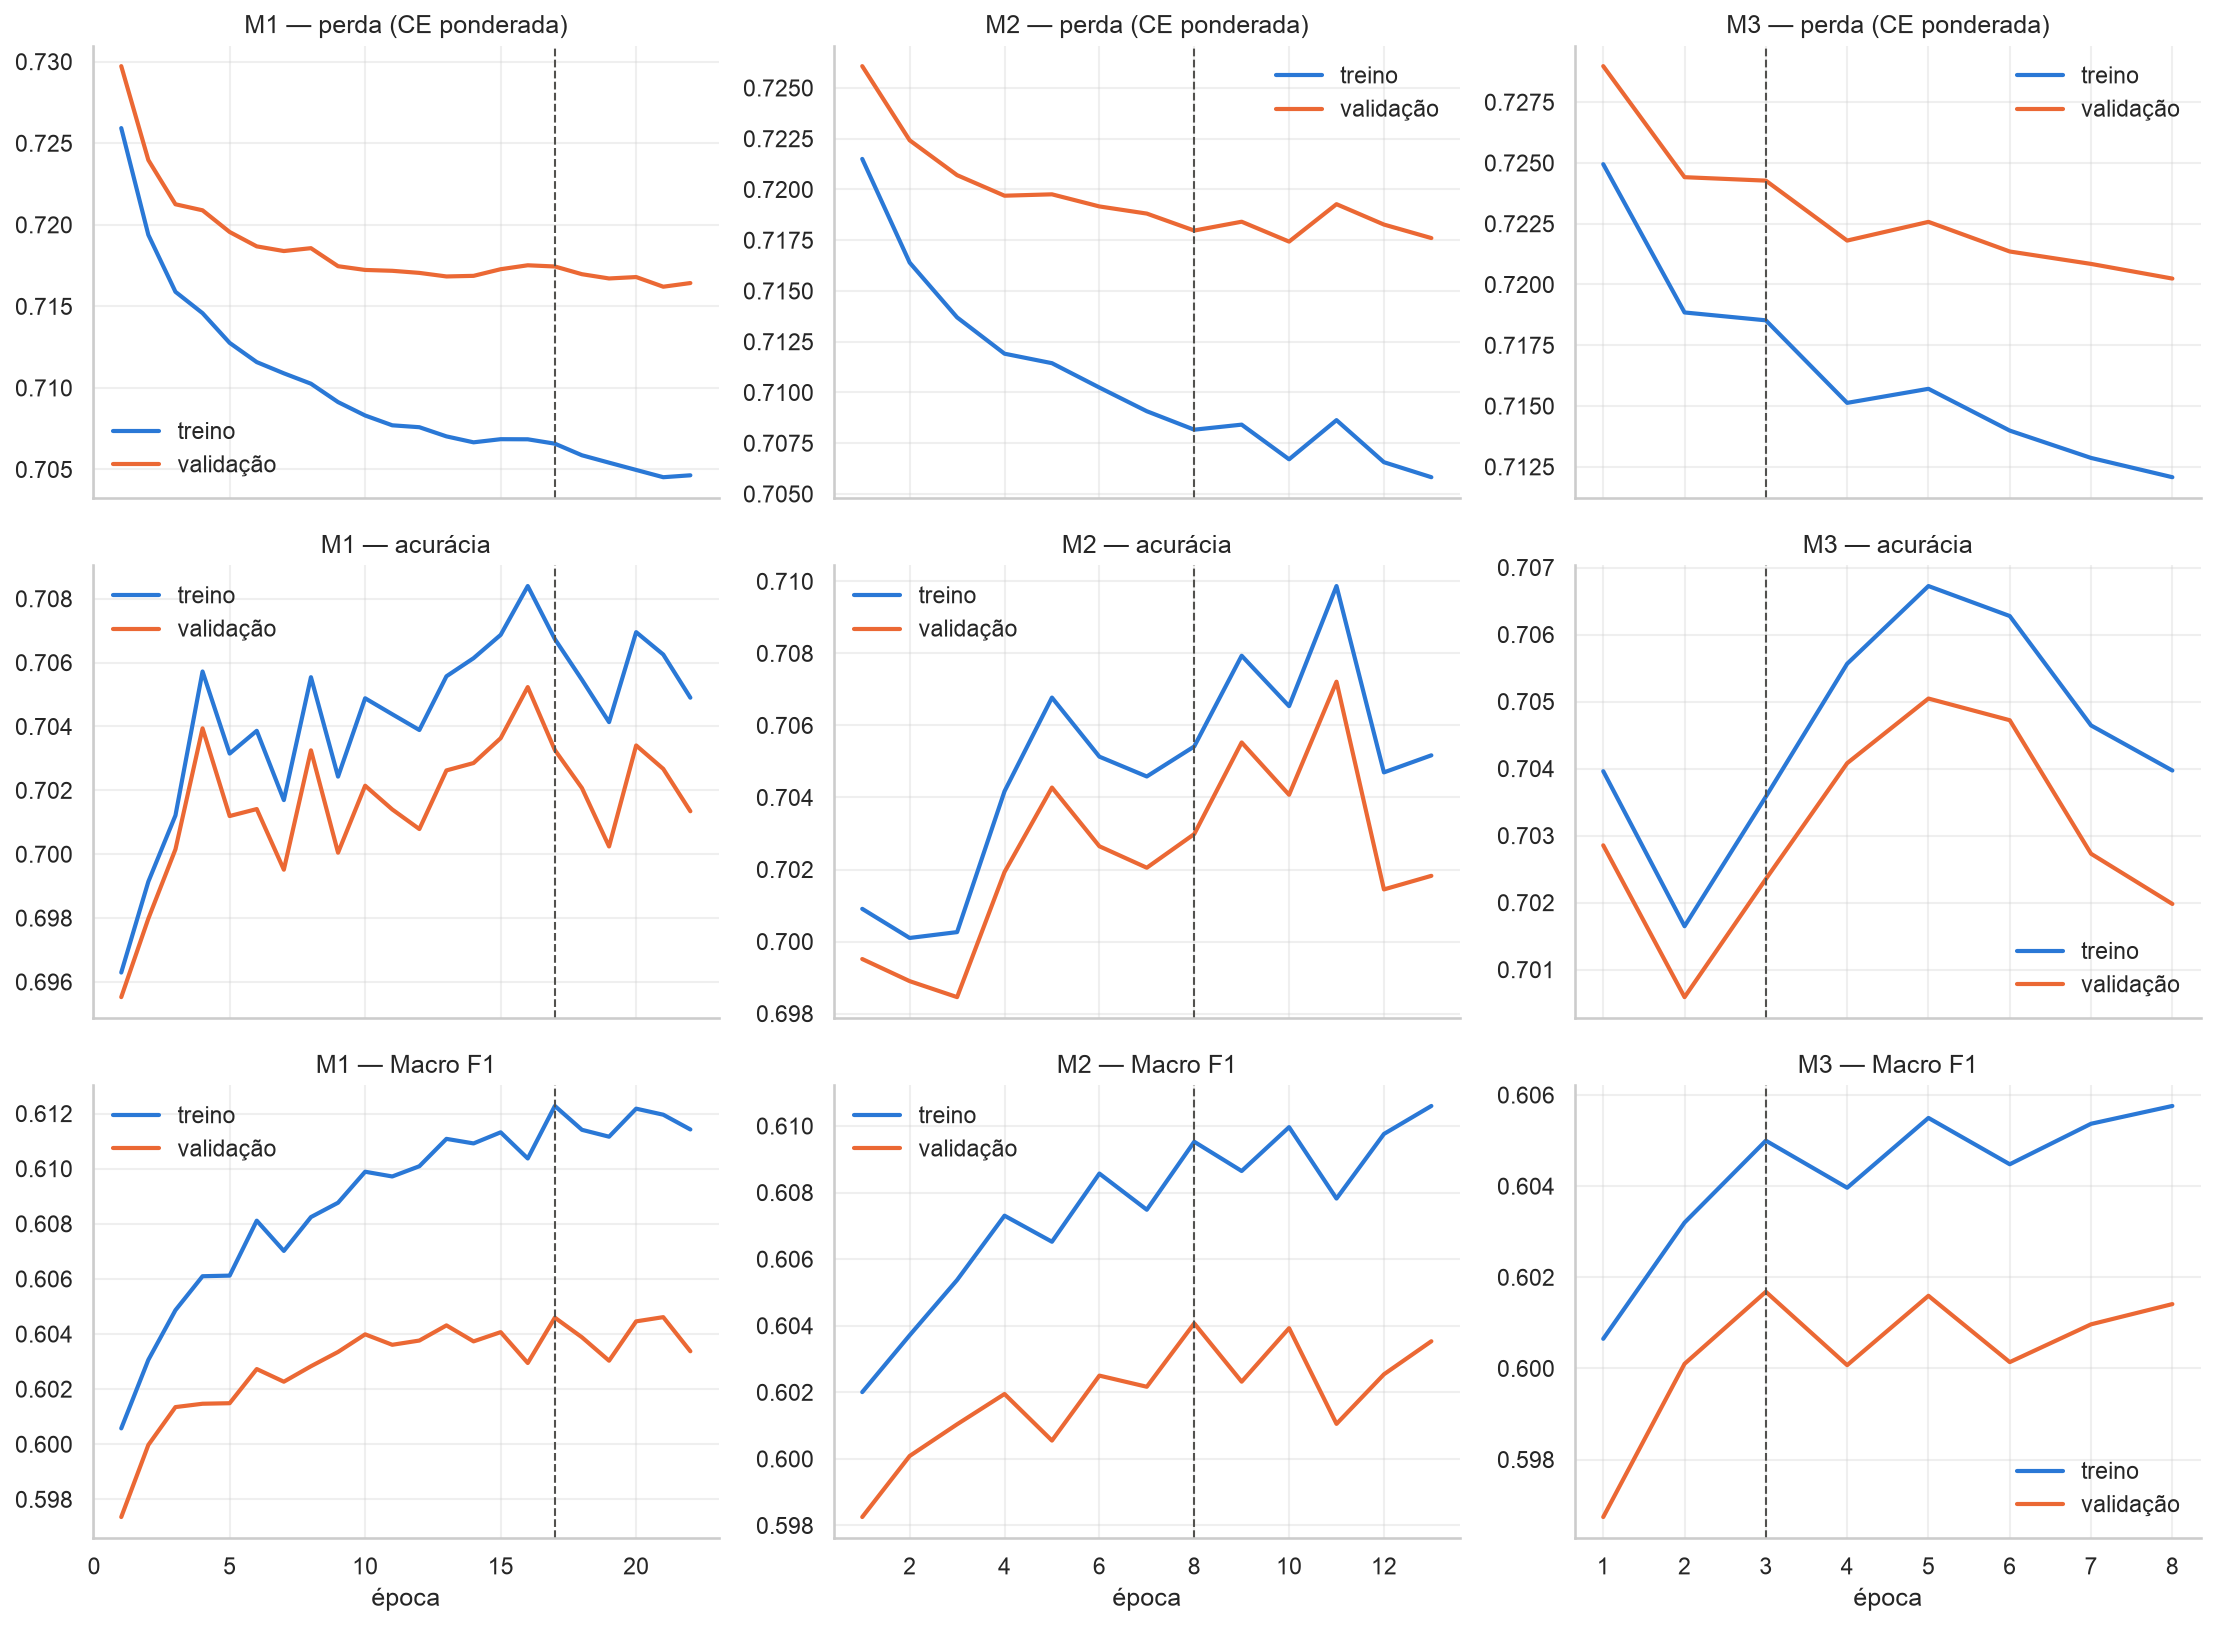
\includegraphics[width=0.42\textwidth]{figuras/12_curvas_treino_validacao}
  \caption{À esquerda, matrizes de confusão do M1 no teste, em contagens e normalizadas pela classe real; à direita, perda, acurácia e Macro F1 por época dos finalistas, com a linha tracejada na melhor época}
  \label{fig:confusao}
  \fontefig{Elaborado pelo autor}
\end{figure}

\section{Curvas de treino e validação}
\label{sec:curvas}

Nas curvas dos três finalistas (Figura~\ref{fig:confusao}, à direita), a perda de treino e a de validação caem juntas, e o Macro F1 de validação para de melhorar e oscila (melhor época 17 no M1, 8 no M2 e 3 no M3), o que dispara a parada antecipada. O sobreajuste é leve: o \textit{gap} de Macro F1 na melhor época fica entre 0,003 e 0,008, menor no M3, que tem o maior dropout. Não há subajuste: o teto de cerca de 70\% de acurácia vem das entradas (Seção~\ref{sec:baselines}), não da capacidade da rede. Já o \textit{recall} de 40\% nos fatais é o ponto de operação dos pesos de classe, não um teto: um peso maior elevaria o \textit{recall} à custa da precisão.


\section{Comparação com \textit{baselines} e ablação por grupo de entradas}
\label{sec:baselines}

A MLP supera a regressão logística (com \texttt{C} escolhido na validação) em 1,8 p.p. de acurácia e de Macro F1 (Tabela~\ref{tab:baselines}): um ganho real, mas pequeno, vindo da combinação não linear das mesmas entradas. A ablação (Figura~\ref{fig:ablacao-grupos}) mostra de onde vem o desempenho: só com o contexto da via a MLP empata com a tabela de frequências (52,9\%) e nunca prevê fatal; local e horário acrescentam 2,9 p.p.; o relato do solicitante acrescenta 14,6 p.p. e é o que faz a classe fatal ser reconhecida (\textit{recall} de 0 para 0,40). As entradas pesam muito mais que a arquitetura; o efeito isolado de \texttt{macro\_causa}, a única do grupo que não vem do solicitante, não foi medido.

\begin{table}[!htbp]
\caption{Comparação com \textit{baselines} no teste}
\label{tab:baselines}
\begin{center}
\footnotesize
\begin{tabularx}{\textwidth}{Y c c}
\hline
\textbf{Modelo} & \textbf{Acurácia} & \textbf{Macro F1} \\ \hline
Classe majoritária & 0,484 & 0,217 \\
Sorteio proporcional às classes & 0,455 & 0,334 \\
Tabela de frequências só com o contexto da via (414 combinações) & 0,529 & 0,361 \\
Regressão logística (12 entradas, $C = 1$) & 0,685 & 0,588 \\
\textbf{MLP M1} & \textbf{0,703} & \textbf{0,607} \\ \hline
\end{tabularx}
\end{center}
\fontetab{Elaborado pelo autor}
\end{table}

\begin{figure}[!htbp]
  \centering
  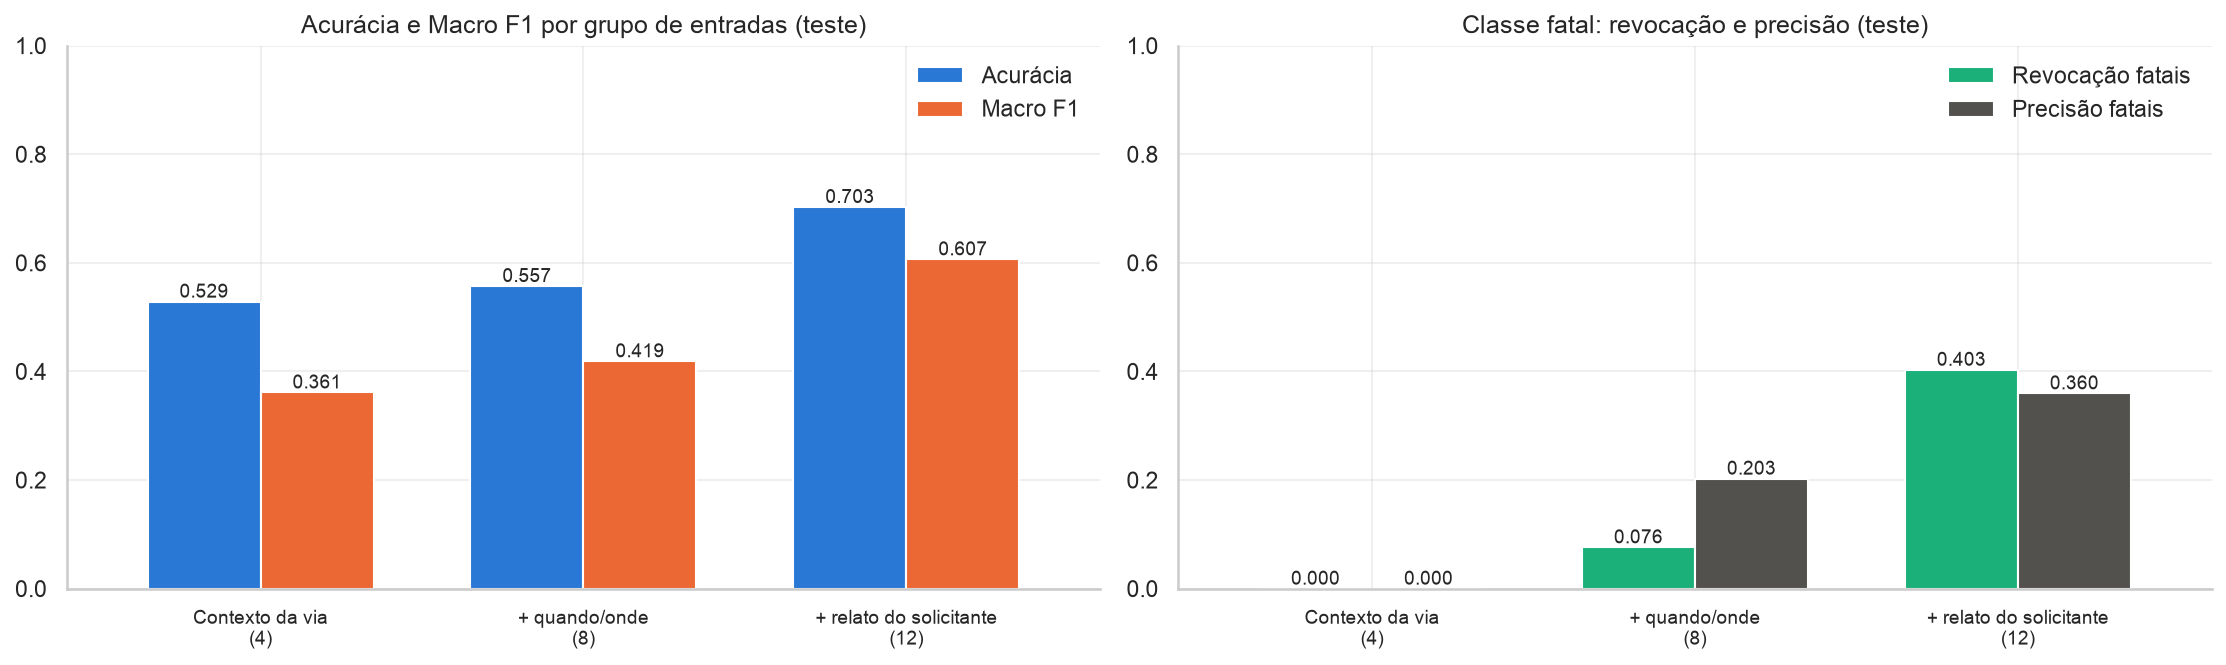
\includegraphics[width=0.7\textwidth]{figuras/14_ablacao_grupos_entradas}
  \caption{Arquitetura de M1 treinada com grupos crescentes de entradas (teste)}
  \label{fig:ablacao-grupos}
  \fontefig{Elaborado pelo autor}
\end{figure}
